\section{Life Cycle of a Query}
\label{sec:qdep}
%  \mnote{4.4 describes the workflows in the architecture, ie how components are used to implement
% desired functionality; this is also when you introduce algorithms etc.}  \mnote{Description of the
% steps involved in the deployment of a query}
This section describes the workflow of a query, from when it is submitted to when it starts processing.
It shows how different aspects of the system are realised by describing the process of instantiating,
deploying and connecting a query.
First, a query plan is submitted in XML format. Based on this, the system creates a set of customised
operator instances. After a query has been instantiated, it is broken down into subqueries employing a
flexible partitioning policy. Each subquery is deployed on a processing node, chosen from a set of
suitable candidates provided by the oracle. Finally, the different subqueries are connected to each
other, tuples start flowing from the input providers and the processing begins.
Figure~\ref{fig:qdep} shows the steps involved in the deployment of a query.
% ----------  OVERVIEW  -----------------
\begin{myenumerate}
  \item First, the query graph is submitted in XML format. It contains the query specification
  with a list of tuples and operators to be used. It also has information about the links among
  operators. 
  \item The \emph{submitter} compiles and instantiates the XML query specification, creating the tuples
  and operator objects. Next, it starts a \emph{coordinator}, which is the entity in charge of deploying
  and monitoring the status of the query.
  \item The \emph{coordinator} creates $N$ subqueries from the original query graph according to a user
  defined partitioning policy. Next, it contacts the \emph{oracle} to obtain a set of $N$ nodes for
  deployment.\\
  \item The \emph{oracle} returns a list of the $N$ most suitable nodes available for deployment. This
  choice is dictated by a system-wide policy, such as choosing the least loaded nodes or nodes with a low
  network latency between them.
  \item Once the \emph{coordinator} receives this information, it proceeds by deploying the individual
  subqueries onto the provided \emph{processing nodes}.
  \item Each \emph{processing node} instantiates the assigned subquery and connects the query,
  establishing the required remote network connections between the operators.
  \item Finally, the \emph{input provider} operators connect to the external sources and start feeding
  tuples to the query. The query is then deployed and starts processing.
\end{myenumerate}
\begin{figure}[t!]
	\centering
	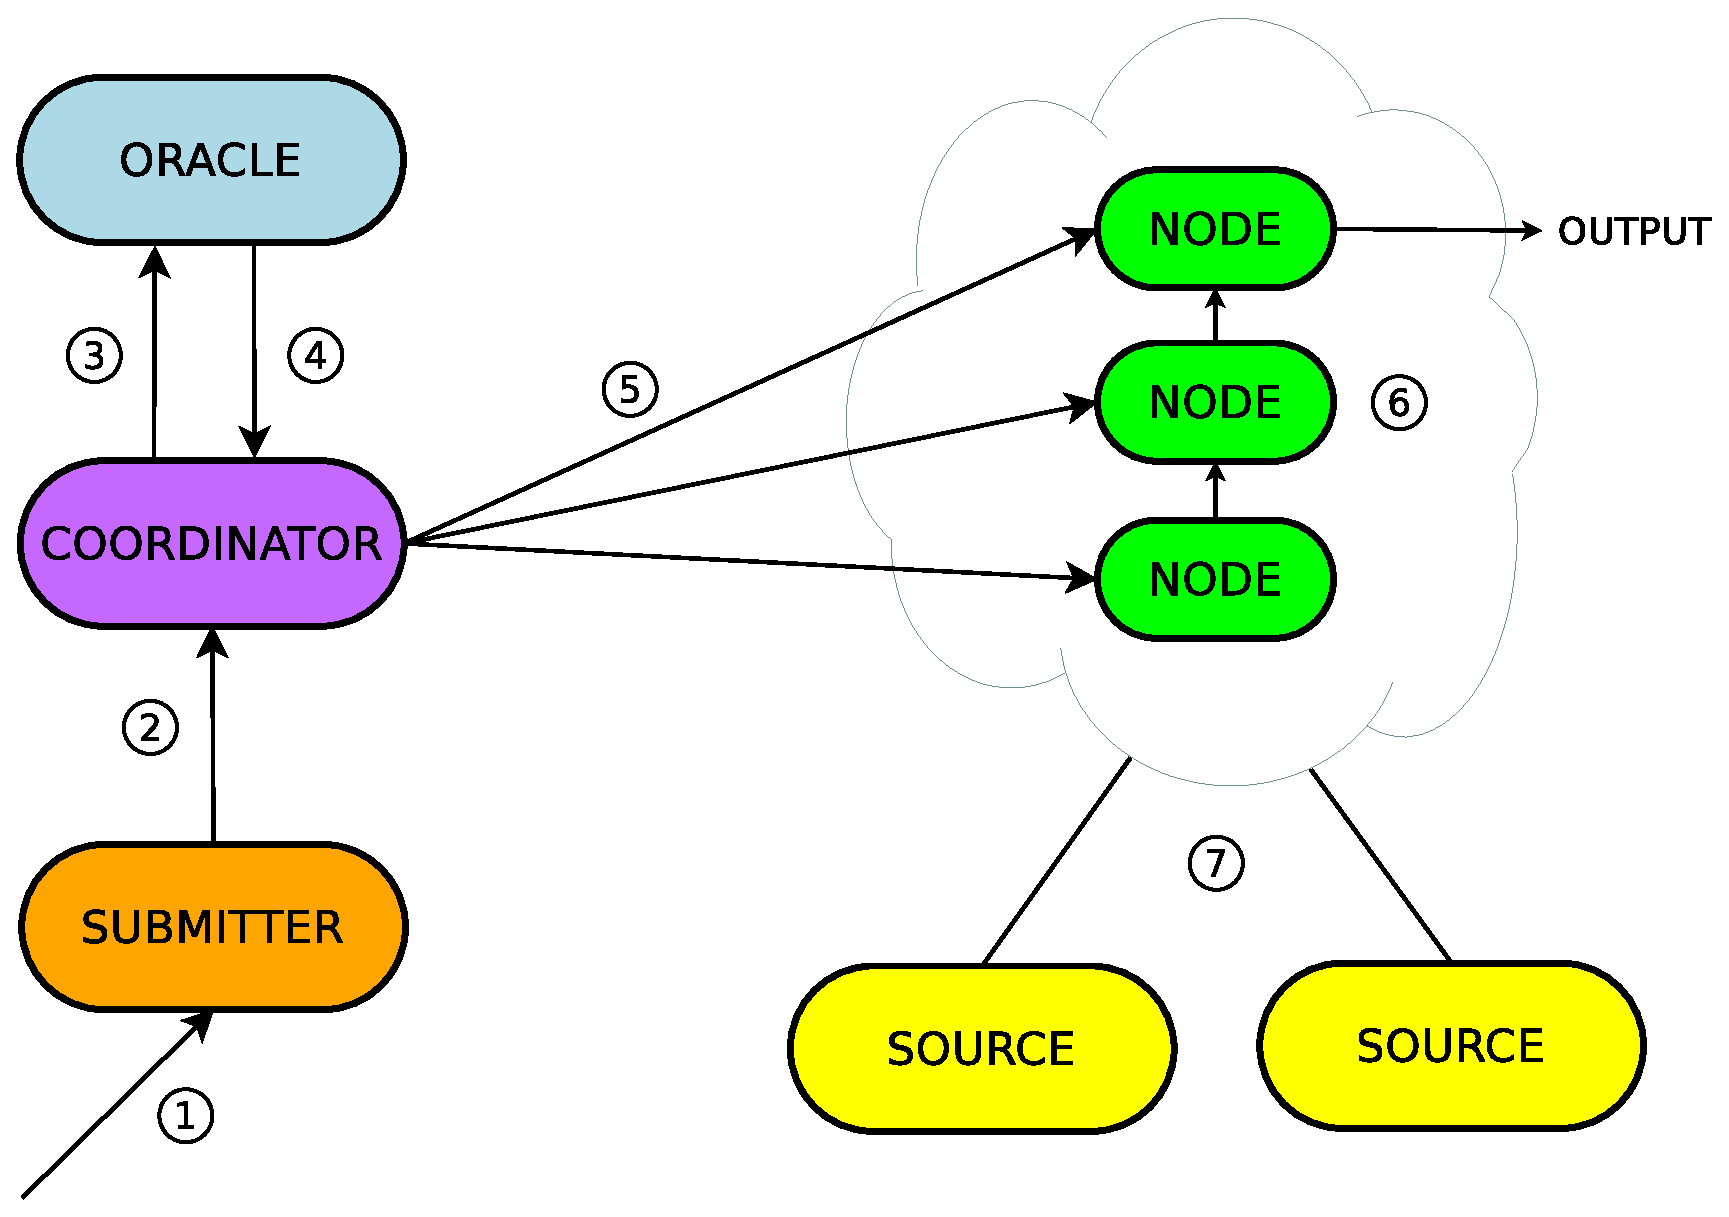
\includegraphics[width=0.6\textwidth]{img/tesi/query_deployment.eps} 
	\caption{Steps involved in the deployment of a query.}
	\label{fig:qdep}
\end{figure} 
% ---------- SUBMISSION -----------------
\vspace{-15pt}
\subsection{Submission of Queries}
\label{sec:qsub}
\vspace{-5pt}
%\mnote{should include ``compilation'' of tuples and ops }
The life cycle of a query begins with the submission of its query plan by a user. This is done through
the \emph{submitter} component. It interprets the XML query specification and compiles a set of custom
operator instances. Operators and tuples are compiled at run-time for better performance. The next
paragraphs introduce the concept of \emph{compiled} operators and tuples and how they are realised in the
DISSP design.
	
\subsubsection*{Compiled Operators and Tuples}
\label{sec:templates}
In the DISSP system, tuples and operators are implemented as \emph{compiled Plain Old Java
Objects (POJO)}~\cite{pojo}.
This choice was made taking performance into consideration because other options, based for example on
\emph{reflection}, are slow and can cause a potential performance bottleneck. To
instantiate a custom tuple or operator object based on the query requirements, a text \textit{template}
is completed with the information contained in the XML query specification that describes the query
producing a new Java source file, which is then compiled to bytecode by a run-time compiler.
\paragraph{XML Query Representation.} Queries are submitted to the system in an XML representation.
An XML query file contains the complete description of the query. It specifies what kind of tuples
are processed and provides a description of the \emph{tuple schemas} so that operators are aware of the
number, type and name of the fields contained in the tuples that they process. It also includes the list
of operators implementing the query semantics. Each operator is represented by an XML block, containing
its description. \\
An operator needs to be specialised before it can be used in a query. A
generic implementation is provided in a \emph{template file}, which acts as a blueprint for the operator.
It is then completed with the data included in the XML block, allowing the correct instantiation of the
operator: its \emph{name, parameters} and an indication of its \emph{subsequent operator}. An
operator either declares itself as a \emph{terminal} operator by having no subsequent operators, or as an
\emph{intermediate} operator with its output used as input to another operator.\\
Based on this information, the system reconstructs the complete query graph.
The XML query representation is used to generate a complete set of Java source files
that define the customised tuples and operators that are used in the query. These files are then compiled
and instantiated so that the query can begin processing. 

\paragraph{Templates.} Semi-complete \textrm{Java} source files represent the skeleton of a class and
are used for the efficient instantiation of customised \textit{tuples} and \textit{operators}.
All tuples share common characteristics but differ in the number of fields, their names and types. The
same is true for all operators that belong to the same type. For example, all average operators have the
same processing semantics but have different names and types of the fields to be averaged. \\
A generic blueprint for these operators comes from the generalisation of a specific instance, in which
specific names and types are replaced by textual \emph{placeholders}.
Using the information contained in the XML query description, it is possible to substitute these
placeholders with the correct details, transforming a template into a complete \textrm{Java} source file
ready for compilation.
Placeholders are all capitals keywords preceded by a dollar sign in the form ``\texttt{\$PLACEHOLDER}''.
They are replaced using the information provided in the XML file describing the query and then compiled
into actual Java objects with the required characteristics.
For this transformation, the system uses a \textit{CharSequenceCompiler}, which takes as input a string
with the content of a completed \textrm{template} file and produces an instance of a customised object.
This means that the system operates on compiled bytecode, which combines a high execution efficiency with
the flexibility of working with customised versions of tuples and operators tailored to the query
requirements.
% \lstset{ basicstyle=\ttfamily, columns=fixed, showstringspaces=false,
% commentstyle=\color{white}\upshape }  \lstdefinelanguage{XML} { morestring=[b]", %morestring=[s]{>}{<},
% morecomment=[s]{<?}{?>}, stringstyle=\color{BrickRed}, identifierstyle=\color{NavyBlue},
% keywordstyle=\color{ForestGreen}, morekeywords={type,name}% list your attributes here }
% \noindent\begin{minipage}{\textwidth} \begin{lstlisting}[language=XML,label=lst:opxml,caption=XML
% description of an Average operator] <operator name="MyAvgCpu" type="Average"> <next name="MyOutput"/>
% <parameter name="tuple"    value="simpleSchemaONE" /> <parameter name="field"    value="cpu"/>
% <parameter name="groupby"  value="idx"/> <operator> \end{lstlisting} \end{minipage} 
% \exblock{Listing~\ref{lst:opxml} shows the XML description of an \emph{Average} operator. In the first
% line the operator is characterized as being an instance of class ``Average'', described in the
% correspondant .template file, and it is given the name of ``MyAvgCpu'. Then there is the declaration of
% a \emph{next} operator, this means that this is not a terminal operator and thus its output should be
% delivered to a single local operator named ``MyOutput''. Next are 3 parameter definitions, in the form
% $\langle name, value \rangle$. The system will look for the ``\$NAME'' placeholder and will replace it
% with the string given by ``value''. Once the substitution has taken place, the .template file becomes a
% complete .java source file and is then compiled by the \emph{CharSequenceCompiler}.}
%\clearpage
% ---------------------------------
Tuples are also implemented using a template file. A parent class called \texttt{Tuple} is provided that
contains the basic processing logic common to all tuples, and every tuple class is derived from it.
In the XML query description, the user specifies a schema and a name for the tuples that are used by the
query, and the system creates a new tuple class with the required name and fields. The generic
tuple template file is then completed, substituting the placeholders with the provided data,
thus producing the Java source file of the new tuple class.

Listing~\ref{lst:tuplexml} shows the XML description of a Tuple object with three fields: a
\texttt{long} field for the timestamp named \textit{ts} and two \texttt{double} fields, one with a
numerical identifier \textit{idx} and the other for a temperature reading \textit{tmp}. These values are
inserted in the tuple template in correspondence with the ``\texttt{\$FIELD}'' placeholder, transforming
it into a complete Java source file. As a result, the compiled object contains three public fields with
the types and names from the XML listing.
 \lstset{
  basicstyle=\singlespacing\ttfamily, columns=fixed, showstringspaces=false,
  commentstyle=\color{white}\upshape }

\lstdefinelanguage{XML}
{
  morestring=[b]",
  %morestring=[s]{>}{<},
  morecomment=[s]{<?}{?>},
  stringstyle=\color{BrickRed},
  identifierstyle=\color{NavyBlue},
  keywordstyle=\color{ForestGreen}, 
  morekeywords={type,name}% list your attributes here
}
\begin{lstlisting}[language=XML,label=lst:tuplexml,caption=XML description of a Tuple]
	<schema name="simpleSchemaONE">
	    <field type="long"   name="ts"  />
	    <field type="double" name="idx" />
	    <field type="double" name="tmp" />  
	</schema>
\end{lstlisting}
 
%--------------------------------- 
Listing~\ref{lst:opxml} shows the XML description of an average operator. In the first line the
operator is defined as being an instance of class \texttt{Average}, described in the corresponding
template file, and it is given the name \texttt{MyAvgCpu}. 

Next, there is the declaration of a \textit{subsequent} operator, which means that this is not a terminal
operator. Its output should be delivered to a single local operator named \texttt{MyOutput}. 
This is followed by three parameter definitions in the form of $\langle name,
value \rangle$. The system considers the \texttt{\$NAME} placeholder and replaces it with the string
given by \texttt{value}. After this substitution, the template file becomes a
complete Java source file and is compiled by the \textit{CharSequenceCompiler}.
\lstset{
  basicstyle=\ttfamily\singlespacing,
  columns=fixed,
  showstringspaces=false,
  commentstyle=\color{white}\upshape
}

\lstdefinelanguage{XML}
{
  morestring=[b]",
  %morestring=[s]{>}{<},
  morecomment=[s]{<?}{?>},
  stringstyle=\color{BrickRed},
  identifierstyle=\color{NavyBlue},
  keywordstyle=\color{ForestGreen}, 
  morekeywords={type,name}% list your attributes here
}
\noindent\begin{minipage}{\textwidth}
\begin{lstlisting}[language=XML,label=lst:opxml,caption=XML description of an Average operator]
	<operator name="MyAvgCpu" type="Average">
	    <next name="MyOutput"/>
	    <parameter name="tuple"    value="simpleSchemaONE" />
	    <parameter name="field"    value="cpu"/>
	    <parameter name="groupby"  value="idx"/>
	<operator>
\end{lstlisting}
\end{minipage}	
%\clearpage
The DISSP system provides a number of general-purpose operator templates: \textit{window operators}
provide transformations over windows, holding the input of an operator until a certain condition is
reached; \textit{I/O operators} act as gateways to the system and provide the conversion from
external to a system tuple representation (and vice versa); \textit{network operators} support
inter-node communication so that a query can be partitioned and distributed across several nodes;
and \textit{\mbox{data manipulation operators}} are used to process the data and are equivalent to the
\textit{relation-to-relation} operators in CQL.

% ---------- PARTITIONING -----------------
\subsection{Partitioning of Queries}
\label{sec:qpart}
After a query was instantiated based on its XML representation, it is broken down into chunks called
\emph{subqueries}. These are computationally less intensive than the complete query and can be deployed
across a set of \emph{processing nodes}. The partitioning process can follow different strategies. 
This section presents two policies: one that takes into account the processing
\emph{load} of the newly created partitions and another that multiplexes particularly heavy
partitions over several nodes, executing them in parallel according to a horizontal partitioning
approach.
\vspace{-10pt}
\paragraph*{Load-Aware Partitioning.}
%\todo{figure load-aware}  
The partitioning of a query graph can follow a strategy that groups operators with similar processing
loads.
Such a \emph{load-aware} strategy tries to obtain subqueries with similar costs in order to spread evenly
the processing load. It is similar to the one described in \cite{borealis-load}.
Since the query partitioning occurs before the query is deployed, the system estimates the cost of an
operator based on its expected \emph{input rate} and \emph{load coefficient}.\\
The expected input rate is calculated for an operator by analysing its direct predecessors in the query
graph and their window operators. The estimate can be more precise in the case of \emph{aggregate
operators}, such as average, because they produce a single output every time that they are triggered. For
\emph{filters}, the estimate is more difficult and must take their selectivity into account. \\ 
The load coefficient of an operator has to be determined offline and estimates the computational
complexity of the operator. A synthetic load of fixed size is input to the operator on a testbed machine
and its CPU load is measured. \\
By multiplying the input rate and the load coefficient, it is possible to
estimate the future load of an operator. The initial partitioning can then divide the query graph
evenly. Note that this should only be thought of as a starting point to be augmented with the run-time
migration of operators or subqueries. This accounts for inaccuracies in the initial estimates. 
\vspace{-10pt}
\paragraph*{Horizontal Partitioning}

The cost of a query is not only determined by the number of operators that it employs. Even queries with
a simple query graph can be computationally expensive due to a high rate of incoming tuples or
the complexity of an operator. In such cases, the partitioning of the query it is not limited to
the grouping of operators into subqueries but includes the rewriting of the query graph. The costly
operator, or subquery, is decomposed so that multiple copies of it can run in parallel on several
processing nodes.
The original input data is split by a \emph{router} operator that sends the chunks in turn to the nodes
hosting the decomposed operator copies.
This approach performs a horizontal scale out of the operator. The output of these operator copies is
sent to a collector operator, which finalises the processing to achieve the original semantics of the
unpartitioned operator.

For example, a costly \emph{average} operator could be decomposed into three copies, each
calculating the average for a $1/3$ of the input. The final average is then calculated by the collector
based on the partial averages.
Other operators, such as \emph{filter}, do not need a further collector phase, and only take a union of
the partial results to generate the final output. 

\begin{figure}[t!]
	\centering	
	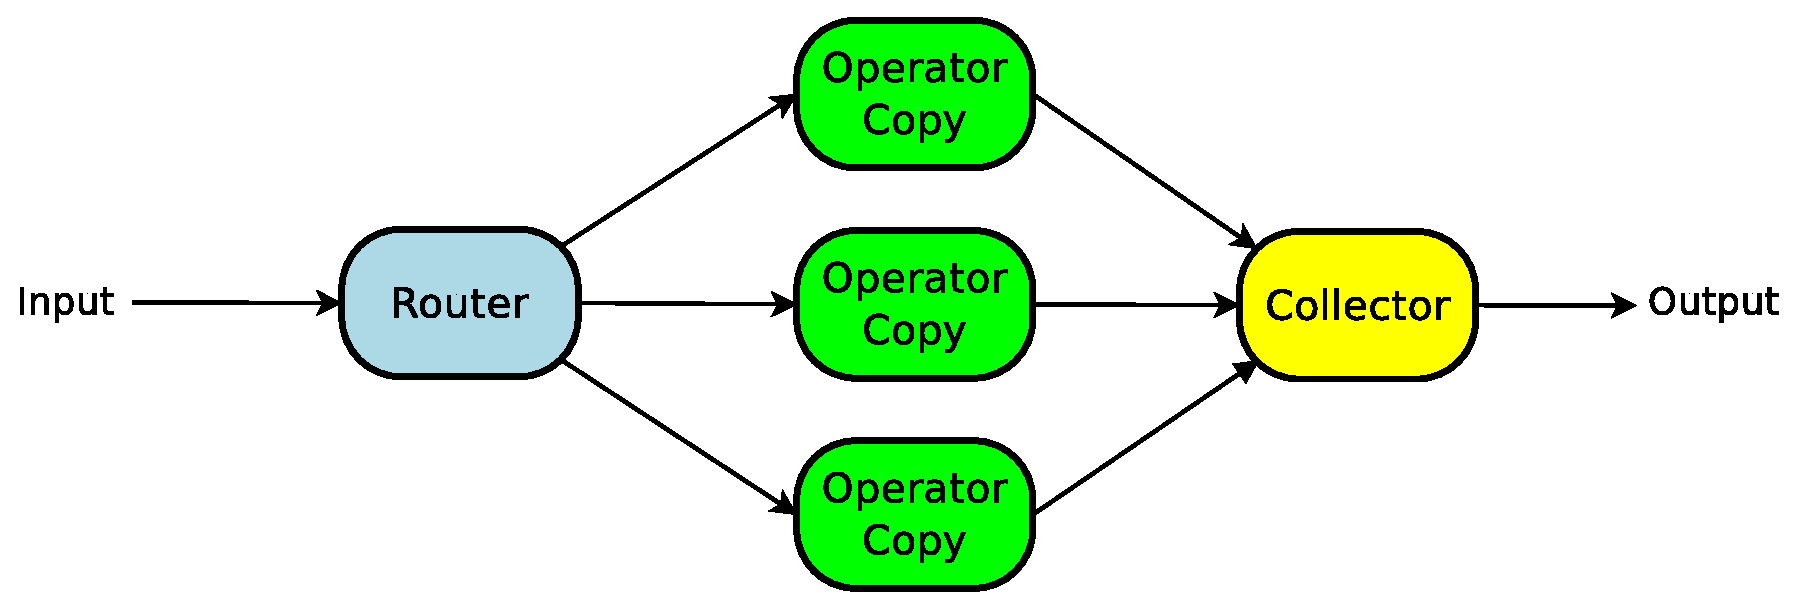
\includegraphics[width=0.8\textwidth]{img/tesi/map-reduce2}
	\caption{Horizontal partitioning of an operator. }
	\label{fig:mr-part}
\end{figure}

Figure~\ref{fig:mr-part} shows the modified query graph of a query rewritten using the
horizontal partitioning strategy. The original query with one expensive operator is transformed so that
three copies of the operators run on different processing nodes. A round-robin router operator evenly
splits the incoming tuples among them. A final replica of the operator, an aggregate in this case,
collects the partial results and outputs the final value. 
\begin{comment}	


% ---------- DEPLOYMENT -----------------
\subsection{Deployment of Queries}

After being partitioned into subqueries, a query is ready to be deployed. 



% ---------- CONNECTION -----------------
\subsection{Connection of Queries}
\label{sec:qsub}
	
\mnote{should include connection and start up of queries}

\begin{figure}
	\centering	
	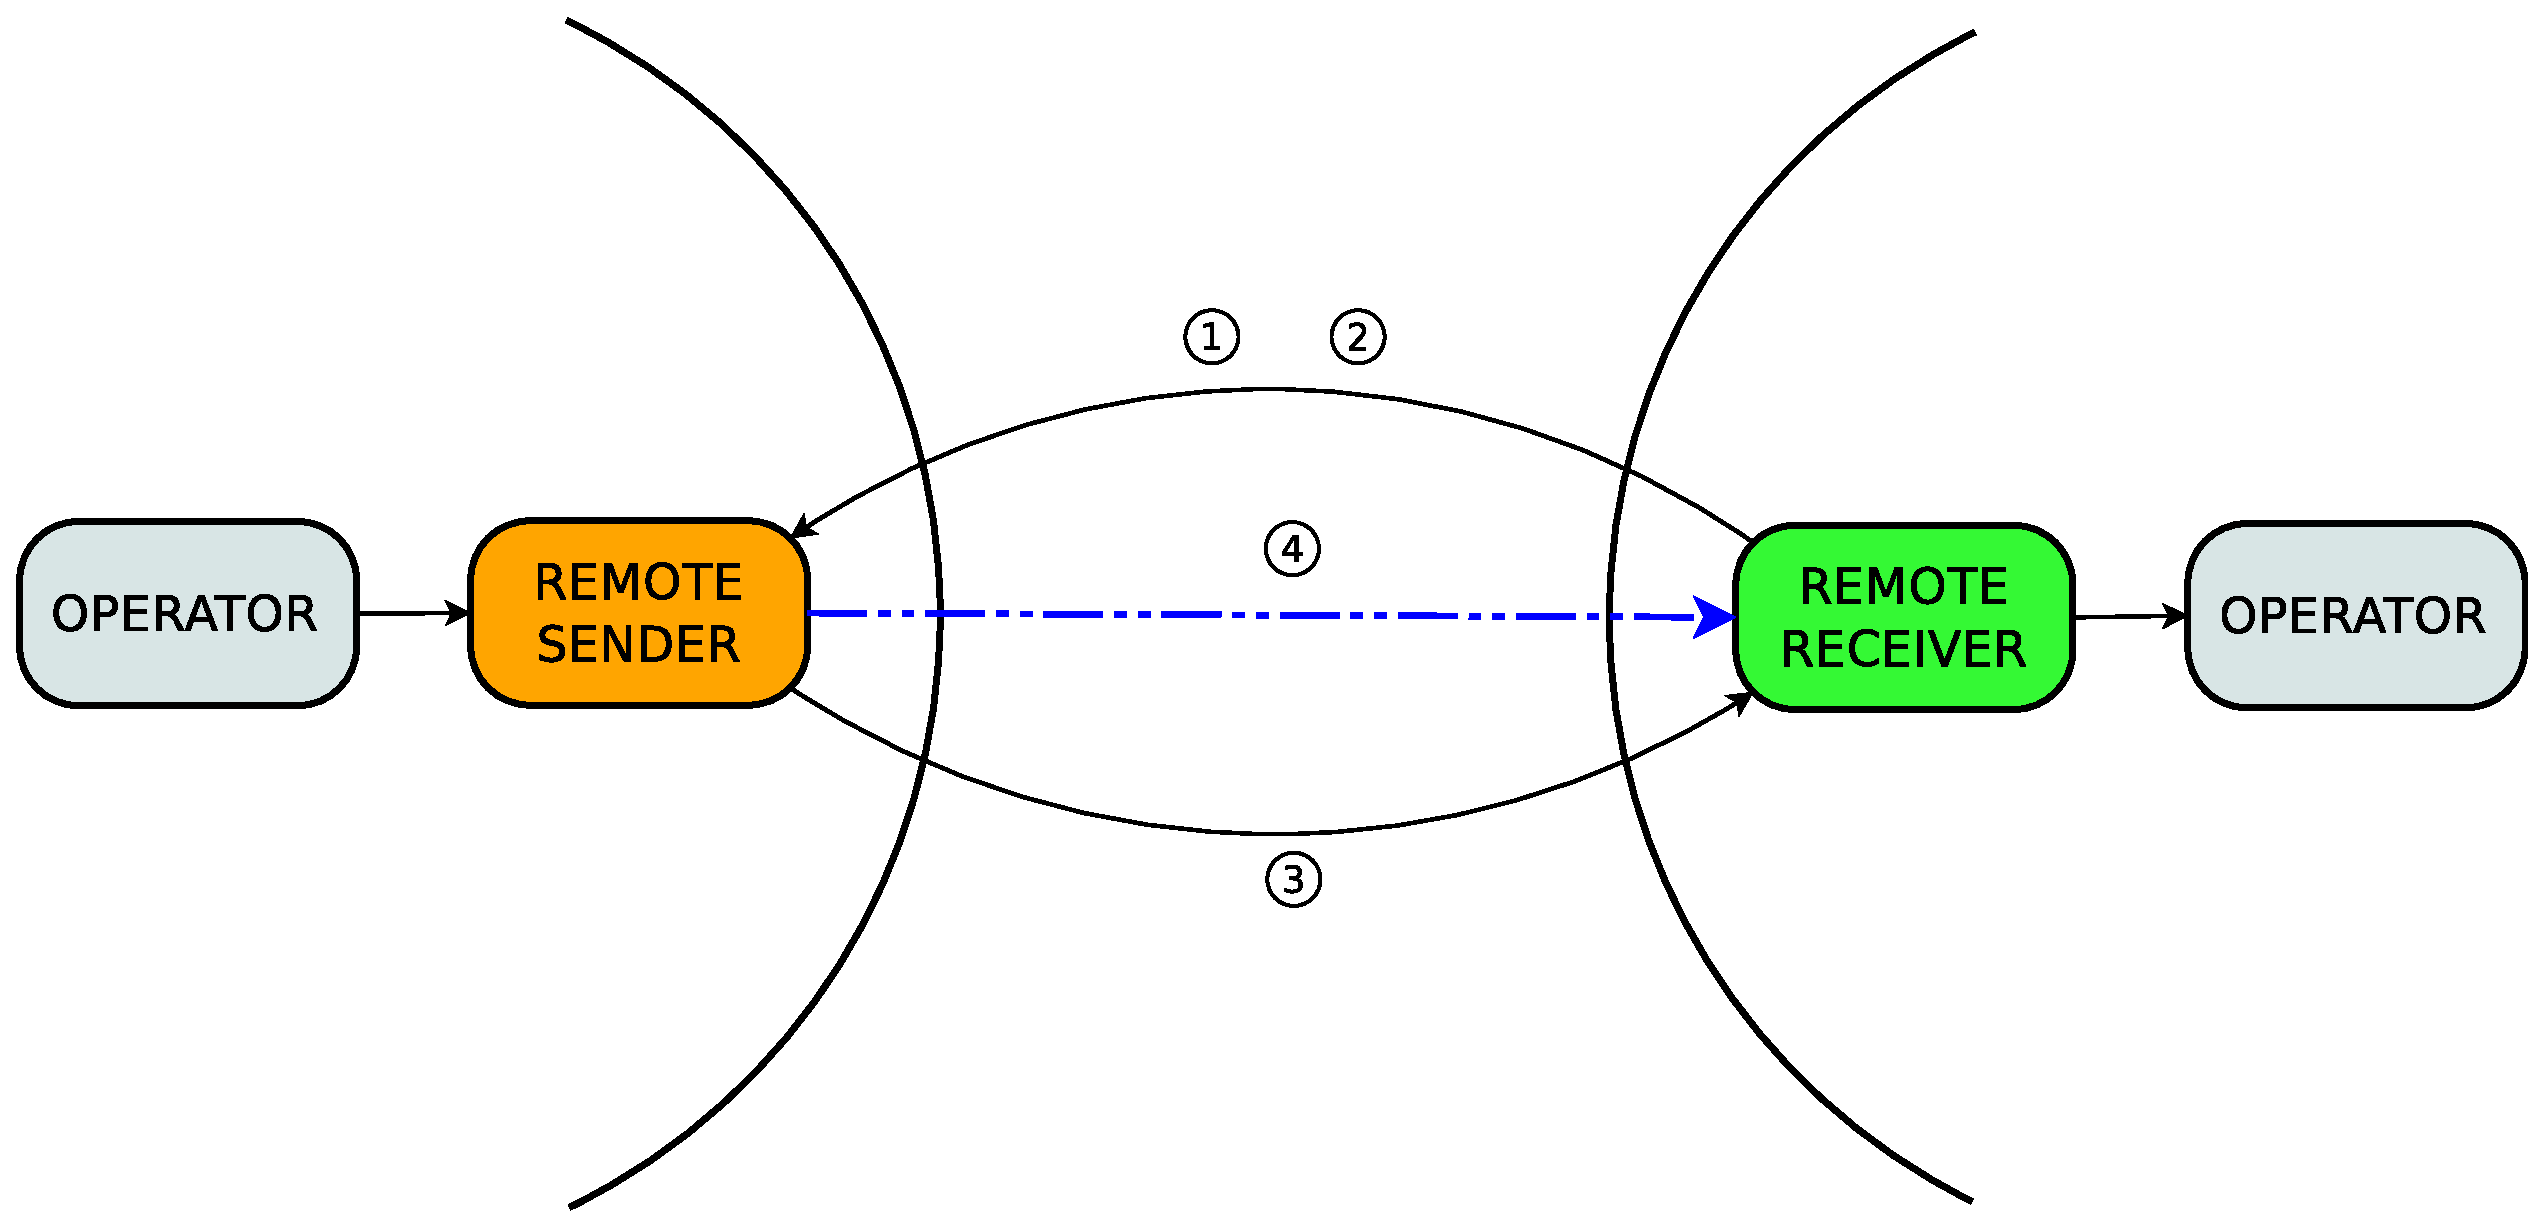
\includegraphics[width=0.8\textwidth]{img/tesi/remote_connection.eps}
	\caption{Remote connection of 2 operators}
	\label{fig:remconn}
\end{figure}
	
\end{comment}


